\documentclass[10pt]{beamer}

\beamertemplatenavigationsymbolsempty

\usepackage{colortbl}

\newcommand\lo{\ensuremath{\boldsymbol{-}}}
\newcommand\hi{\ensuremath{\boldsymbol{+}}}

\title{Factorial Designs}
\author{BIOE 498/598 PJ}
\date{Spring 2021}

\begin{document}
\frame{\titlepage}


\begin{frame}{What is a factorial design?}

A factorial design studies multiple factors set at discrete intervals.

\pause
\bigskip
A design with $k$ factors set at $L$ levels is called an $L^k$ factorial design.

\pause
\bigskip
A factorial design includes runs with every combination of factors set at every level.

	
\end{frame}

\begin{frame}{Sample factorial designs}

\begin{columns}

\begin{column}{0.3\textwidth}
\begin{center}
$2^2$ Factorial design\\
\begin{tabular}{cc}
$x_1$ & $x_2$ \\
\hline
\lo & \lo \\
\hi & \lo \\
\lo & \hi \\
\hi & \hi \\
 & \\
 & \\
 & \\
 & \\
 & \\
\end{tabular}
\end{center}
\end{column}

\begin{column}{0.3\textwidth}
\begin{center}
$2^3$ Factorial design\\
\begin{tabular}{ccc}
$x_1$ & $x_2$ & $x_3$ \\
\hline
\lo & \lo & \lo \\
\hi & \lo & \lo \\
\lo & \hi & \lo \\
\hi & \hi & \lo \\
\lo & \lo & \hi \\
\hi & \lo & \hi \\
\lo & \hi & \hi \\
\hi & \hi & \hi \\
 & \\
\end{tabular}
\end{center}
\end{column}

\begin{column}{0.3\textwidth}
\begin{center}
$3^2$ Factorial design\\
\begin{tabular}{cc}
$x_1$ & $x_2$ \\
\hline
\lo & \lo \\
0 & \lo \\
\hi & \lo \\
\lo & 0 \\
0 & 0 \\
\hi & 0 \\
\lo & \hi \\
0 & \hi \\
\hi & \hi \\
\end{tabular}
\end{center}
\end{column}

\end{columns}
	
\end{frame}


\begin{frame}{Why do we use factorial designs?}

\begin{itemize}
\item Factorial designs find better optima.
\item Factorial designs are more efficient.
\item Factorial designs make better estimates of effect sizes.
\end{itemize}

\end{frame}

\begin{frame}{Why do we use factorial designs?}

\begin{itemize}
\item
  \textbf{Factorial designs find better optima.}
\item
  Factorial designs are more efficient.
\item
  Factorial designs make better estimates of effect sizes.
\end{itemize}

\end{frame}

\begin{frame}{What is a factorial design?}

\begin{figure}
\centering
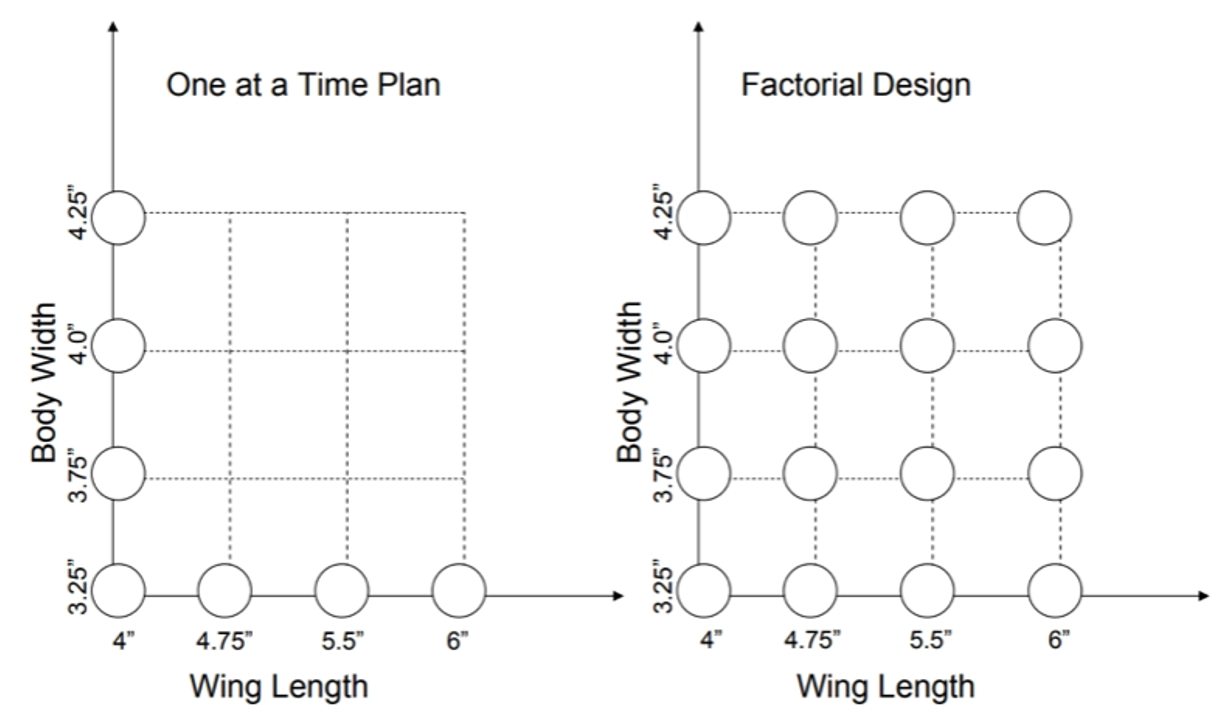
\includegraphics[width=4in]{figures/factorial1.png}
\end{figure}

\end{frame}

\begin{frame}{Factorial designs find better optima}

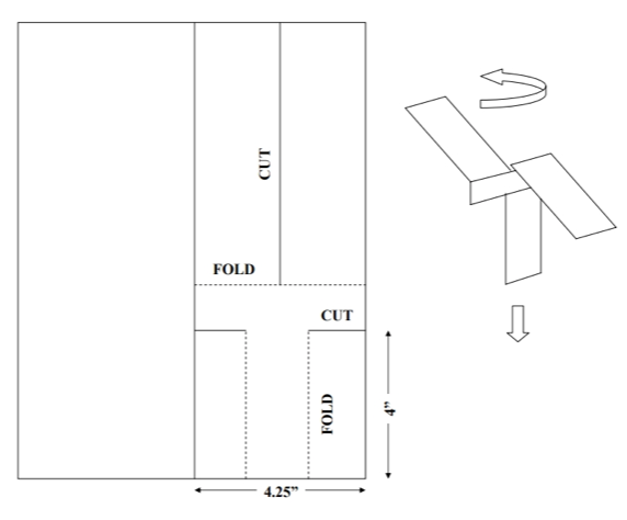
\includegraphics[width=2in]{figures/factorial2-1.png}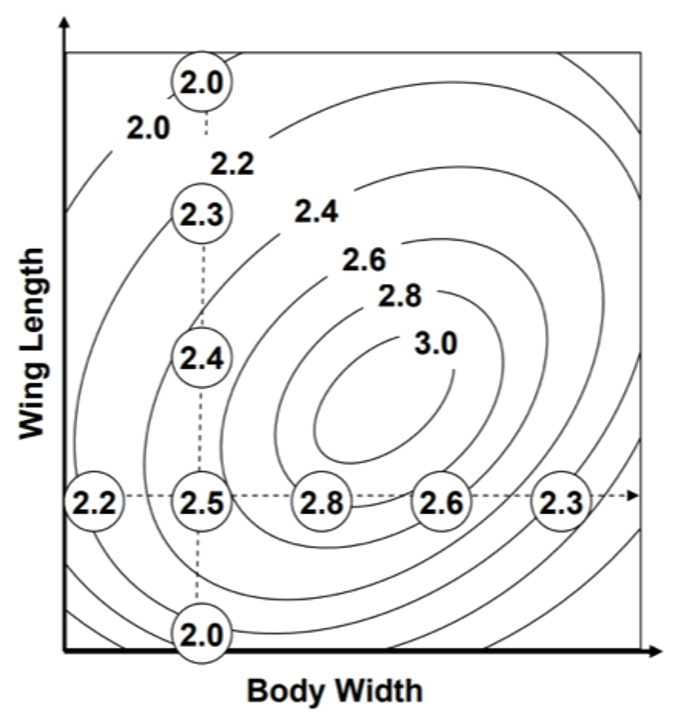
\includegraphics[width=2.5in]{figures/factorial2-3.png}

\end{frame}

\begin{frame}{The problem with OFAT: Interactions}
\centering
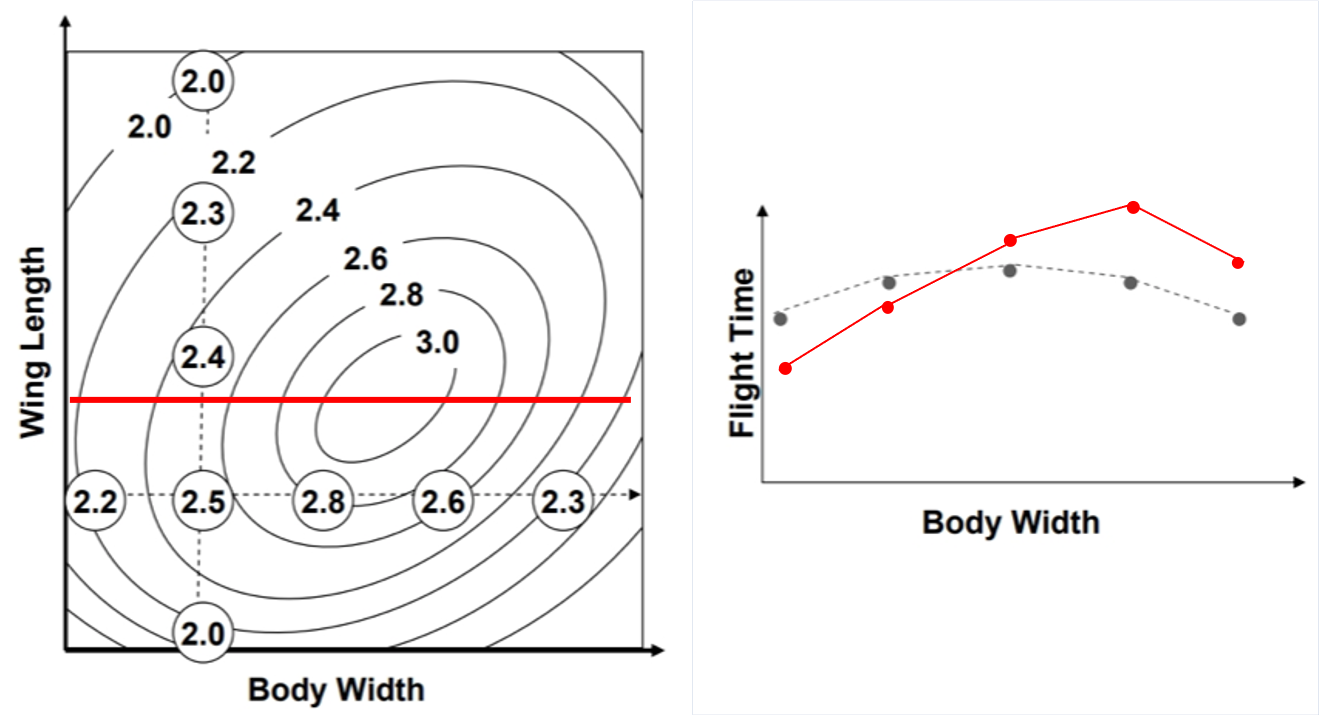
\includegraphics[width=4in]{figures/factorial5.png}

\end{frame}

\begin{frame}{Using interaction plots for diagnosis}
\centering
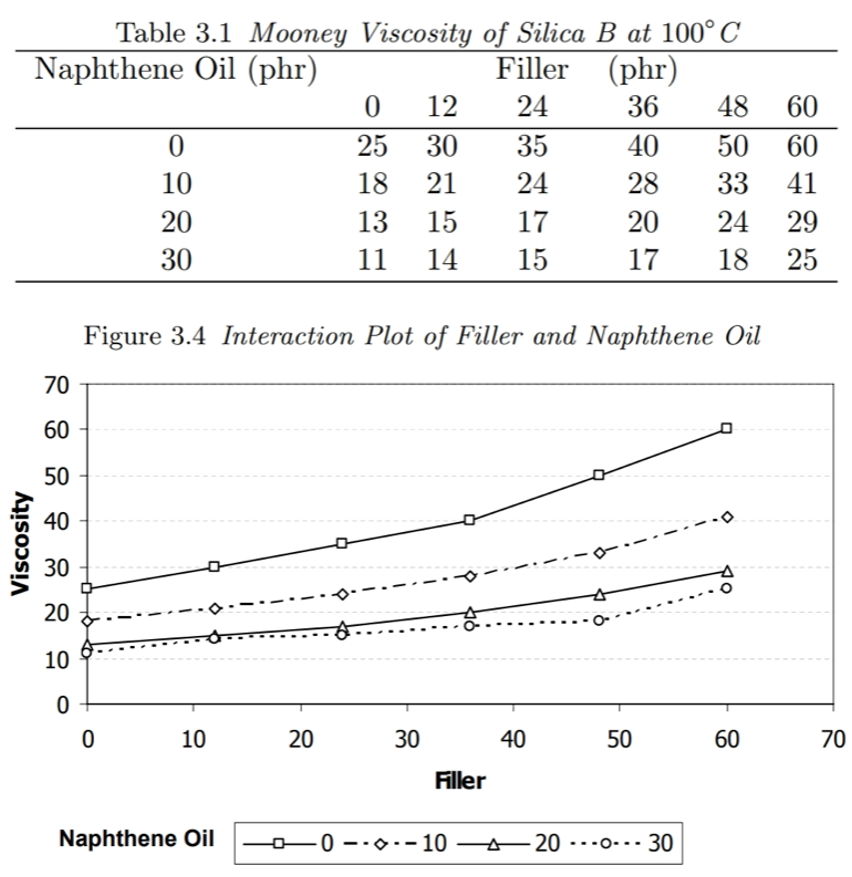
\includegraphics[width=3in]{figures/factorial6.png}

\end{frame}

\begin{frame}{Why do we use factorial designs?}

\begin{itemize}
\item
  Factorial designs find better optima.
\item
  \textbf{Factorial designs are more efficient.}
\item
  Factorial designs make better estimates of effect sizes.
\end{itemize}

\end{frame}

\begin{frame}{Factorial designs seem \emph{less} efficient\ldots{}}

Imagine an experiment with four factors, each with two levels (\(-\),
\(+\)). We want three replicates for each level.

\medskip

One Factor at a Time Design

\begin{itemize}
\item
  3 runs at level (\(-\))
\item
  4 factors \(\times\) 3 runs at (\(+\)) = 12 runs
\item
  \textbf{15 total runs}
\end{itemize}

Factorial Design

\begin{itemize}
\item
  \textbf{$2^4 = \textbf{16}$ total runs}
\end{itemize}

\end{frame}

\begin{frame}{\ldots{}until you look at the designs}

\begin{columns}

\begin{column}{0.45\textwidth}
\begin{center}
OFAT design
\begin{tabular}{cccc}
$x_1$ & $x_2$ & $x_3$ & $x_4$ \\
\hline
\lo & \lo & \lo & \lo \\
\lo & \lo & \lo & \lo \\
\lo & \lo & \lo & \lo \\
\hi & \lo & \lo & \lo \\
\hi & \lo & \lo & \lo \\
\hi & \lo & \lo & \lo \\
\lo & \hi & \lo & \lo \\
\lo & \hi & \lo & \lo \\
\lo & \hi & \lo & \lo \\
\lo & \lo & \hi & \lo \\
\lo & \lo & \hi & \lo \\
\lo & \lo & \hi & \lo \\
\lo & \lo & \lo & \hi \\
\lo & \lo & \lo & \hi \\
\lo & \lo & \lo & \hi \\
 \phantom{\lo} & & & \\
\end{tabular}
\end{center}
\end{column}

\begin{column}{0.45\textwidth}
\begin{center}
Factorial design
\begin{tabular}{cccc}
$x_1$ & $x_2$ & $x_3$ & $x_4$ \\
\hline
\lo & \lo & \lo & \lo \\
\hi & \lo & \lo & \lo \\
\lo & \hi & \lo & \lo \\
\hi & \hi & \lo & \lo \\
\lo & \lo & \hi & \lo \\
\hi & \lo & \hi & \lo \\
\lo & \hi & \hi & \lo \\
\hi & \hi & \hi & \lo \\
\lo & \lo & \lo & \hi \\
\hi & \lo & \lo & \hi \\
\lo & \hi & \lo & \hi \\
\hi & \hi & \lo & \hi \\
\lo & \lo & \hi & \hi \\
\hi & \lo & \hi & \hi \\
\lo & \hi & \hi & \hi \\
\hi & \hi & \hi & \hi \\
\end{tabular}
\end{center}
\end{column}

\end{columns}

\end{frame}

\begin{frame}{Factorial designs give more replicates per run}
\protect\hypertarget{factorial-designs-give-more-replicates-per-run}{}

A factorial design in \(n\) variables has \(2^n\) runs, but \(2^{n-1}\)
replicates at each level (\ensuremath{\boldsymbol{-}},
\ensuremath{\boldsymbol{+}}).

\pause
\bigskip

Imagine a design with \(n\) variables at \(k\) levels.

After the initial design, adding another replicate requires

\begin{itemize}
\item
  \(nk\) runs for a OFAT design
\item
  \(\sim k\) runs for a factorial design
\end{itemize}

\end{frame}

\begin{frame}{Why do we use factorial designs?}

\begin{itemize}
\item
  Factorial designs find better optima.
\item
  Factorial designs are more efficient.
\item
  \textbf{Factorial designs make better estimates of effect sizes.}
\end{itemize}

\end{frame}

\begin{frame}{What are the other factors doing when \(x_3\) is high?}

\begin{columns}

\begin{column}{0.45\textwidth}
\begin{center}
OFAT design
\begin{tabular}{cccc}
$x_1$ & $x_2$ & $x_3$ & $x_4$ \\
\hline
\lo & \lo & \lo & \lo \\
\lo & \lo & \lo & \lo \\
\lo & \lo & \lo & \lo \\
\hi & \lo & \lo & \lo \\
\hi & \lo & \lo & \lo \\
\hi & \lo & \lo & \lo \\
\lo & \hi & \lo & \lo \\
\lo & \hi & \lo & \lo \\
\lo & \hi & \lo & \lo \\
\rowcolor{pink} \lo & \lo & \hi & \lo \\
\rowcolor{pink} \lo & \lo & \hi & \lo \\
\rowcolor{pink} \lo & \lo & \hi & \lo \\
\lo & \lo & \lo & \hi \\
\lo & \lo & \lo & \hi \\
\lo & \lo & \lo & \hi \\
 \phantom{\lo} & & & \\
\end{tabular}
\end{center}
\end{column}

\begin{column}{0.45\textwidth}
\begin{center}
Factorial design
\begin{tabular}{cccc}
$x_1$ & $x_2$ & $x_3$ & $x_4$ \\
\hline
\lo & \lo & \lo & \lo \\
\hi & \lo & \lo & \lo \\
\lo & \hi & \lo & \lo \\
\hi & \hi & \lo & \lo \\
\rowcolor{pink} \lo & \lo & \hi & \lo \\
\rowcolor{pink} \hi & \lo & \hi & \lo \\
\rowcolor{pink} \lo & \hi & \hi & \lo \\
\rowcolor{pink} \hi & \hi & \hi & \lo \\
\lo & \lo & \lo & \hi \\
\hi & \lo & \lo & \hi \\
\lo & \hi & \lo & \hi \\
\hi & \hi & \lo & \hi \\
\rowcolor{pink} \lo & \lo & \hi & \hi \\
\rowcolor{pink} \hi & \lo & \hi & \hi \\
\rowcolor{pink} \lo & \hi & \hi & \hi \\
\rowcolor{pink} \hi & \hi & \hi & \hi \\
\end{tabular}
\end{center}
\end{column}

\end{columns}
\end{frame}

\begin{frame}{What do the effect sizes estimate?}

For OFAT designs:
\begin{center}
	 $\beta_i$ is the effect of moving $x_i$ from \lo\ to \hi\ \\ \textbf{while all other factors stay at \lo}.
\end{center}

\pause
\bigskip
For factorial designs:
\begin{center}
	 $\beta_i$ is the effect of moving $x_i$ from \lo\ to \hi\ \\ \textbf{averaged over all other factors at all levels}.
\end{center}
	
\end{frame}

\begin{frame}{Factorial designs are nested}

\begin{columns}

\begin{column}{0.3\textwidth}
\begin{center}
Factorial design
\begin{tabular}{cccc}
$x_1$ & $x_2$ & $x_3$ & $x_4$ \\
\hline
\lo & \lo & \lo & \lo \\
\hi & \lo & \lo & \lo \\
\lo & \hi & \lo & \lo \\
\hi & \hi & \lo & \lo \\
\rowcolor{pink} \lo & \lo & \hi & \lo \\
\rowcolor{pink} \hi & \lo & \hi & \lo \\
\rowcolor{pink} \lo & \hi & \hi & \lo \\
\rowcolor{pink} \hi & \hi & \hi & \lo \\
\lo & \lo & \lo & \hi \\
\hi & \lo & \lo & \hi \\
\lo & \hi & \lo & \hi \\
\hi & \hi & \lo & \hi \\
\rowcolor{pink} \lo & \lo & \hi & \hi \\
\rowcolor{pink} \hi & \lo & \hi & \hi \\
\rowcolor{pink} \lo & \hi & \hi & \hi \\
\rowcolor{pink} \hi & \hi & \hi & \hi \\
\end{tabular}
\end{center}
\end{column}

\begin{column}{0.3\textwidth}
\begin{center}
When $x_3 = \lo$
\medskip
\begin{tabular}{cccc}
$x_1$ & $x_2$ & $x_4$ \\
\hline
\lo & \lo & \lo \\
\hi & \lo & \lo \\
\lo & \hi & \lo \\
\hi & \hi & \lo \\
\lo & \lo & \hi \\
\hi & \lo & \hi \\
\lo & \hi & \hi \\
\hi & \hi & \hi \\
\end{tabular}
\end{center}
\end{column}

\begin{column}{0.3\textwidth}
\begin{center}
When $x_3 = \hi$
\medskip
\begin{tabular}{ccc}
$x_1$ & $x_2$ & $x_4$ \\
\hline
\rowcolor{pink} \lo & \lo & \lo \\
\rowcolor{pink} \hi & \lo & \lo \\
\rowcolor{pink} \lo & \hi & \lo \\
\rowcolor{pink} \hi & \hi & \lo \\
\rowcolor{pink} \lo & \lo & \hi \\
\rowcolor{pink} \hi & \lo & \hi \\
\rowcolor{pink} \lo & \hi & \hi \\
\rowcolor{pink} \hi & \hi & \hi \\
\end{tabular}
\end{center}
\end{column}

\end{columns}	
\end{frame}


\end{document}
